
%(BEGIN_QUESTION)
% Copyright 2015, Tony R. Kuphaldt, released under the Creative Commons Attribution License (v 1.0)
% This means you may do almost anything with this work of mine, so long as you give me proper credit

On a job you are asked to disconnect a six-conductor cable from a terminal strip in preparation for that cable's complete removal.  Another technician tells you that the other end of that cable has already been completely disconnected, and therefore there can be no dangerous voltage present on the cable.

Your next step is to confirm the absence of dangerous voltage on the conductors before physically touching any of them.  This confirmation, of course, is done with a voltmeter, and we all know that voltage is measured {\it between two points}.  The question now is, how many different combinations of points must you measure between to ensure there is {\it no} hazardous voltage present?

$$\includegraphics[width=15.5cm]{i04261x01.eps}$$

List all possible pairs of points you should test for voltage between, in order to ensure the conductors are safe for you to touch.  Don't forget to include earth ground as one of those points!

\vskip 80pt

Next, write a mathematical formula to calculate the number of point-pair combinations (i.e. the number of different voltage measurements that must be taken) given $N$ number of connection points in the circuit.

\vfil 

\underbar{file i04261}
\eject
%(END_QUESTION)





%(BEGIN_ANSWER)

This is a graded question -- no answers or hints given!

%(END_ANSWER)





%(BEGIN_NOTES)

Recall that voltage is {\it always} measured between two points.  This means we must find every two-point combination for our meter to test.  Thus, you should check between these point pairs (21 voltage measurements in total):

\begin{itemize}
\item{} 1 to 2
\item{} 1 to 3
\item{} 1 to 4
\item{} 1 to 5
\item{} 1 to 6
\item{} 2 to 3
\item{} 2 to 4
\item{} 2 to 5
\item{} 2 to 6
\item{} 3 to 4
\item{} 3 to 5
\item{} 3 to 6
\item{} 4 to 5
\item{} 4 to 6
\item{} 5 to 6
\item{} 1 to ground
\item{} 2 to ground
\item{} 3 to ground
\item{} 4 to ground
\item{} 5 to ground
\item{} 6 to ground
\end{itemize}

A general formula for calculating the number of voltage measurements to take between $N$ number of points:

$${1 \over 2}(N^2 - N)$$

\vskip 10pt

To be extra-cautious, one should test for both AC voltage and DC voltage, doubling the number of voltage tests!

\vskip 10pt

A good way to approach the problem of deriving a formula is to simplify the problem so that there are fewer points to test between, then gradually increase the number of test points to see how this increase affects the number of necessary tests.  After a few trials of doing this with different numbers of test points, you should begin to see a mathematical pattern leading you to a formula.

The following table shows the relationship between number of test points ($N$) and the number of required voltmeter measurements to cover all possible combinations of two points:

% No blank lines allowed between lines of an \halign structure!
% I use comments (%) instead, so that TeX doesn't choke.

$$\vbox{\offinterlineskip
\halign{\strut
\vrule \quad\hfil # \ \hfil & 
\vrule \quad\hfil # \ \hfil \vrule \cr
\noalign{\hrule}
%
% First row
Test points ($N$) & Number of measurements required \cr
%
\noalign{\hrule}
%
% Another row
2 & 1 \cr
%
\noalign{\hrule}
%
% Another row
3 & 3 \cr
%
\noalign{\hrule}
%
% Another row
4 & 6 \cr
%
\noalign{\hrule}
%
% Another row
5 & 10 \cr
%
\noalign{\hrule}
%
% Another row
6 & 15 \cr
%
\noalign{\hrule}
%
% Another row
7 & 21 \cr
%
\noalign{\hrule}
%
% Another row
8 & 28 \cr
%
\noalign{\hrule}
%
% Another row
9 & 36 \cr
%
\noalign{\hrule}
%
% Another row
10 & 45 \cr
%
\noalign{\hrule}
} % End of \halign 
}$$ % End of \vbox

With each increment of $N$, we see the number of tests growing by a larger degree.  If you look closely at this sequence, it should be apparent that the number of required measurements grows by $N-1$ with each increase in $N$.  Note how with 5 points we require 10 measurements, but with 6 points we require 15 measurements: {\it 5 more than before}.  With 7 points we require 21 measurements: {\it 6 more than before}.

Another pattern which should be apparent by looking at this table is how the number of required measurements are all common multiples of integers: 3 is 3 $\times$ 1; 6 is 3 $\times$ 2; 10 is 5 $\times$ 2; 15 is 5 $\times$ 3.  This clue suggests we might be able to calculate the number of required tests by forming a product (multiplication) of numbers based on the value of $N$.

Let's take the pair of 6, 15 for example: 6 test points requiring 15 measurements.  Is there any way to get 15 out of the number 6 by using multiplication?  We know that 15 is 5 $\times$ 3, and that 5 is one less than 6, while 3 is half of 6.  We may then check to see if other rows in this table seem to follow this same pattern.  7 test points require 21 measurements: one less than 7 is 6, while half of 7 is 3.5, and the product of these (6 $\times$ 3.5) does indeed equal 21.  In fact, we may try this with any entry in the table and get the same result: take one away from $N$, then multiply by one-half of $N$, to get the number of required voltage measurements.

Codifying this in a formula:

$$(N-1){N \over 2}$$

This of course may also be expressed as ${1 \over 2}(N^2 - N)$.


%INDEX% Safety, electrical: voltage testing after lock-out / tag-out

%(END_NOTES)

